\begin{refsection}[research/sugita/group.bib]
\nocite{*}
\chapter{Computational Biophysics Research Team}

\section{Members}

\begin{itemize}
 \item[] Yuji Sugita (Team Leader (Concurrent))*, **
 \item[] Osamu Miyashita (Senior Research Scientist)
 \item[] Jaewoon Jung (Research Scientist)
 \item[] Chigusa Kobayashi (Research Scientist)
 \item[] Yasuhiro Matsunaga (Research Scientist)
 \item[] Hiromi Kano (Assistant)
 \item[] Takaharu Mori (Research Scientist (Concurrent))**
 \item[] Isseki Yu (Research Scientist (Concurrent))**
 \item[] Raimondas Galvelis (Postdoctoral Researcher (Concurrent))**
 \item[] Takao Yoda (Visiting Scientist) ***
 \item[] Mitsunori Ikeguchi (Visiting Scientist)****
 \item[] Naoyuki Miyashita (Visiting Scientist)
 \item[] Michael Feig (Visiting Scientist)
\end{itemize}

* The main affiliation of these people is Laboratory for Biomolecular Function Simulation, Computational Biology Research Core, RIKEN Quantitative Biology Center.

** The main affiliation is RIKEN Theoretical Molecular Science Laboratory.

*** The main affiliation is Nagahama Bio Institute.

**** The main affiliation is Yokohama City University.

\section{Research Activities}

In this team, we have developed GENESIS(Generalized Ensemble Simulation
System) for molecular dynamics simulations. The key features of GENESIS
are that it is highly parallelized for K and other massively parallel
supercomputers and that GENESIS contains a lot of enhanced
conformational sampling methods and various molecular models for
multi-scale and multi-resolution simulations. We have already open the
code of GENESIS as free software under the license of GPLv2 and will
update it every two year by adding new functions and optimizing the code
into K or other computational platforms. These activities are necessary,
in particular, for biological applications, since many interesting
biological phenomena happen on the milliseconds or slower but current
all-atom MD simulations cover only 1-10 microseconds on the
general-purpose supercomputers or GPU clusters. We intend to spread
GENESIS into academia as well as industries as a basic MD program that
is useful for research and development. 

\section{Research Results and Achievements}

\subsection{Developement of GENESIS}

We have already optimized GENESIS for large scale MD simulations on K
computer. In the given fiscal year, we further optimized it by
increasing parallel efficiency and enlarging the available number of
processors. First, we make use of a multiple-program, multiple-data
approach by separating computational resources responsible for real
space and reciprocal space interactions. Second, we assign multiple time
step integrator where time-consuming parts are skipped regularly based
on the multiple-program and multiple-data approach. Our new
implementation was tested on the K computer, and we could obtain very
good performance results for big systems consisting of 1 million, 8.5
million, and 28 million atoms systems just increasing the parallel
efficiencies. One MD cycle with the PME calculations for systems
containing 1 million, 8.5 million, and 28 million atoms could be
finished within 2.8 ms, 5.4 ms, and 8 ms (Figure~\localref{fig:fig01}).

\begin{figure}[tbp]
\centering
  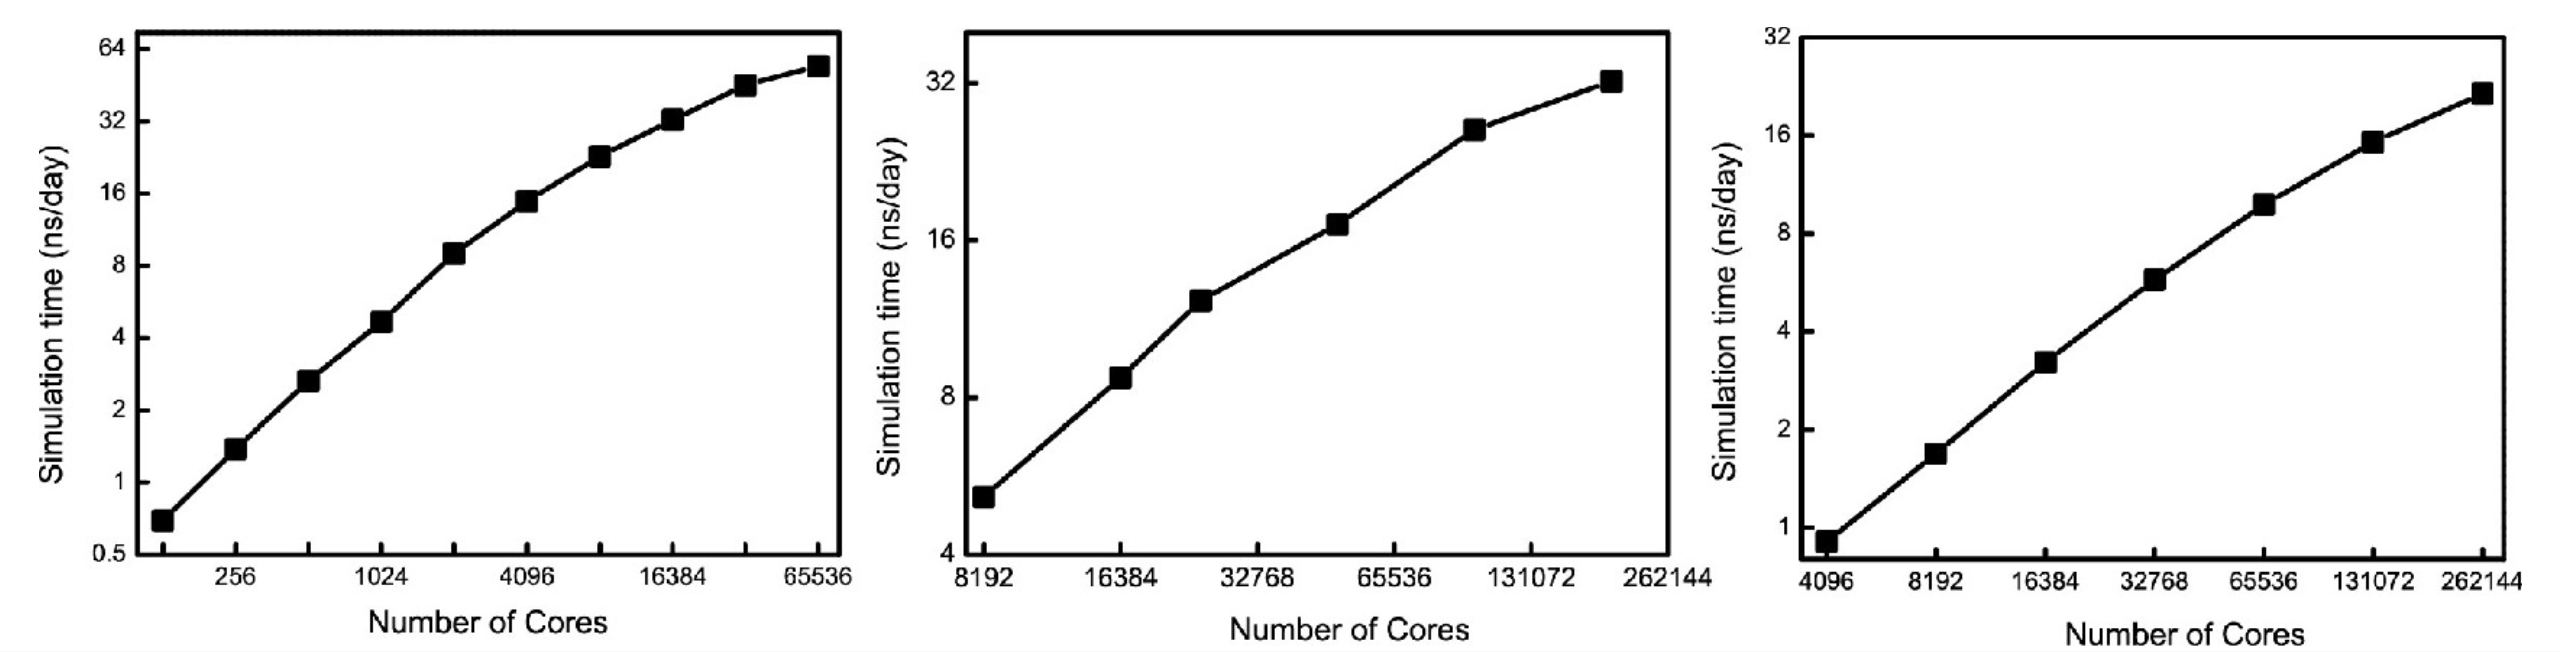
\includegraphics[width=0.8\textwidth,keepaspectratio,natwidth=193,natheight=40]
  {research/sugita/fig01.png}
  \caption{GENESIS performance of 1M (left), 8.5M (middle), and 28M (right) systems}
  \locallabel{fig:fig01}
\end{figure}

\subsection{Multi-resolution simulation methods for reactions couple with large conformational changes}

Recently, experimental studies proposed that large conformational
changes of proteins play important roles on biological functions. The
conformational changes can originate as domain motions, where rigid
structural units (domains) change their positions and/or orientations
with respect to each other through flexible hinges or loops. It is
difficult to investigate atomistic details of multi-domain proteins by
experimental studies. In addition, it is still difficult to simulate
using all-atom MD due to the slow time-scale. To overcome the
difficulties, we have developed multi-resolution simulation method
including the following three steps; 1. Analysis for “dynamic domains”
and the magnitude of local domain motions in a protein through “Motion
Tree”, a tree diagram that describes conformational changes in a
hierarchical manner from two structures. (Koike et al., {\it J. Mol. Biol.},
2014) 2. Development of a structure-based coarse-grained (CG) model
enables a stable and efficient MD simulation from the information of
domain motion obtained by ``Motion Tree''~\cite{Kobayashi01}. The CG
model provides a stable trajectory that is comparable to experimental
studies and long-time all-atom MD simulations. 3. Performing sampling
simulations with the CG model and investigate conformational changes in
response to reactions in biological systems. We examine how many CVs are
required to capture the correct transition-state structure during the
open-to-close motion of adenylate kinase using a coarse-grained model in
the mean forces string method to search the minimum free-energy
pathway~\cite{Kobayashi02}.

\subsection{Systematic evaluation of collective variable choice for describing conformational changes of a protein}

Collective variables (CVs) are often used in molecular dynamics
simulations based on enhanced sampling algorithms to investigate large
conformational changes of a protein. The choice of CVs in these
simulations is essential because it affects simulation results, and
impacts on the free-energy profile, the minimum free-energy pathway
(MFEP), and the transition-state structure. Here, we examine how many
CVs are required to capture the correct transition-state structure
during the open-to-close motion of Adenylate Kinase using a
coarse-grained model in the mean forces string method to search the
MFEP. Various numbers of large amplitude principal components (PCs) are
tested as CVs in the simulations. The incorporation of local coordinates
into CVs, which is possible in higher dimensional CV spaces, is
important for capturing a reliable MFEP. The Bayesian measure proposed
by Best and Hummer is sensitive to the choice of CVs, showing sharp
peaks when the transition-state structure is captured. We thus evaluate
the required number of CVs needed in enhanced sampling simulations for
describing protein conformational changes (Figure~\localref{fig:fig02}~\cite{Matsunaga02}).

\begin{figure}[tbp]
\centering
  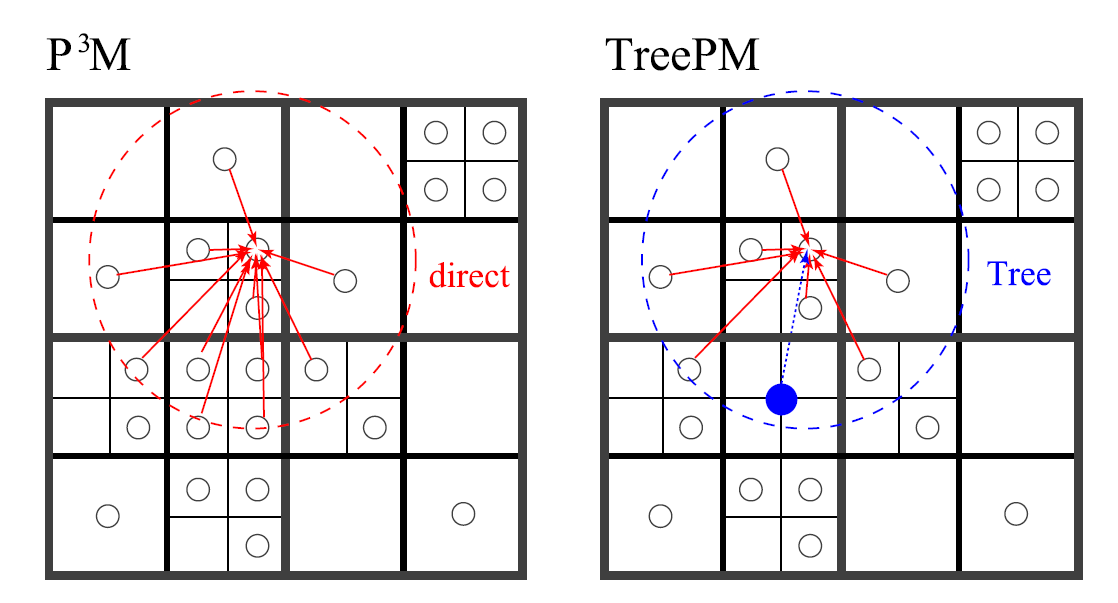
\includegraphics[width=0.8\textwidth,keepaspectratio,natwidth=193,natheight=40]
  {research/sugita/fig02.png}
  \caption{Free-energy landscape in the distances between domains'
 centers of mass. Lines indicate minimum free energy paths calculated in
 2D (dark blue), 3D (light blue), 10D (yellow), and 20D (red) principal
 component spaces.} 
  \locallabel{fig:fig02}
\end{figure}

\subsection{Molecular crowding effect on GTP hydrolysis reaction in Ras-GAP complex}

Macromolecular crowding effects have essential role in biomolecular
system. Such effects have been extensively investigated experimentally,
and also in classical Molecular Dynamics (MD) calculations. However, in
the quantum chemistry level, those effects are not investigated due to
the computational costs and methodological difficulties. In this study,
we studied the molecular crowding effect on the GTP hydrolysis reaction
in Ras-GAP complex by QM/MM RWFE method, which can take crowding effects
into account with a reasonable computational cost. We modeled a crowding
environment by adding 7 BSAs to the system as a crowder, and refined the
reactant and transition states of the hydrolysis reaction by QM/MM RWFE
method, where MD calculations were performed by GENESIS at
K-computer. The structural difference around GTP were not significant
between solution and crowding environment. However, there was a large
difference in the electrostatic potential (ESP) imposed by the
surroundings as shown in Figure~\localref{fig:fig03}. This large ESP
change suggests that there must be significant differences in the free
energy barrier between crowding and solution environments.

\begin{figure}[tbp]
\centering
  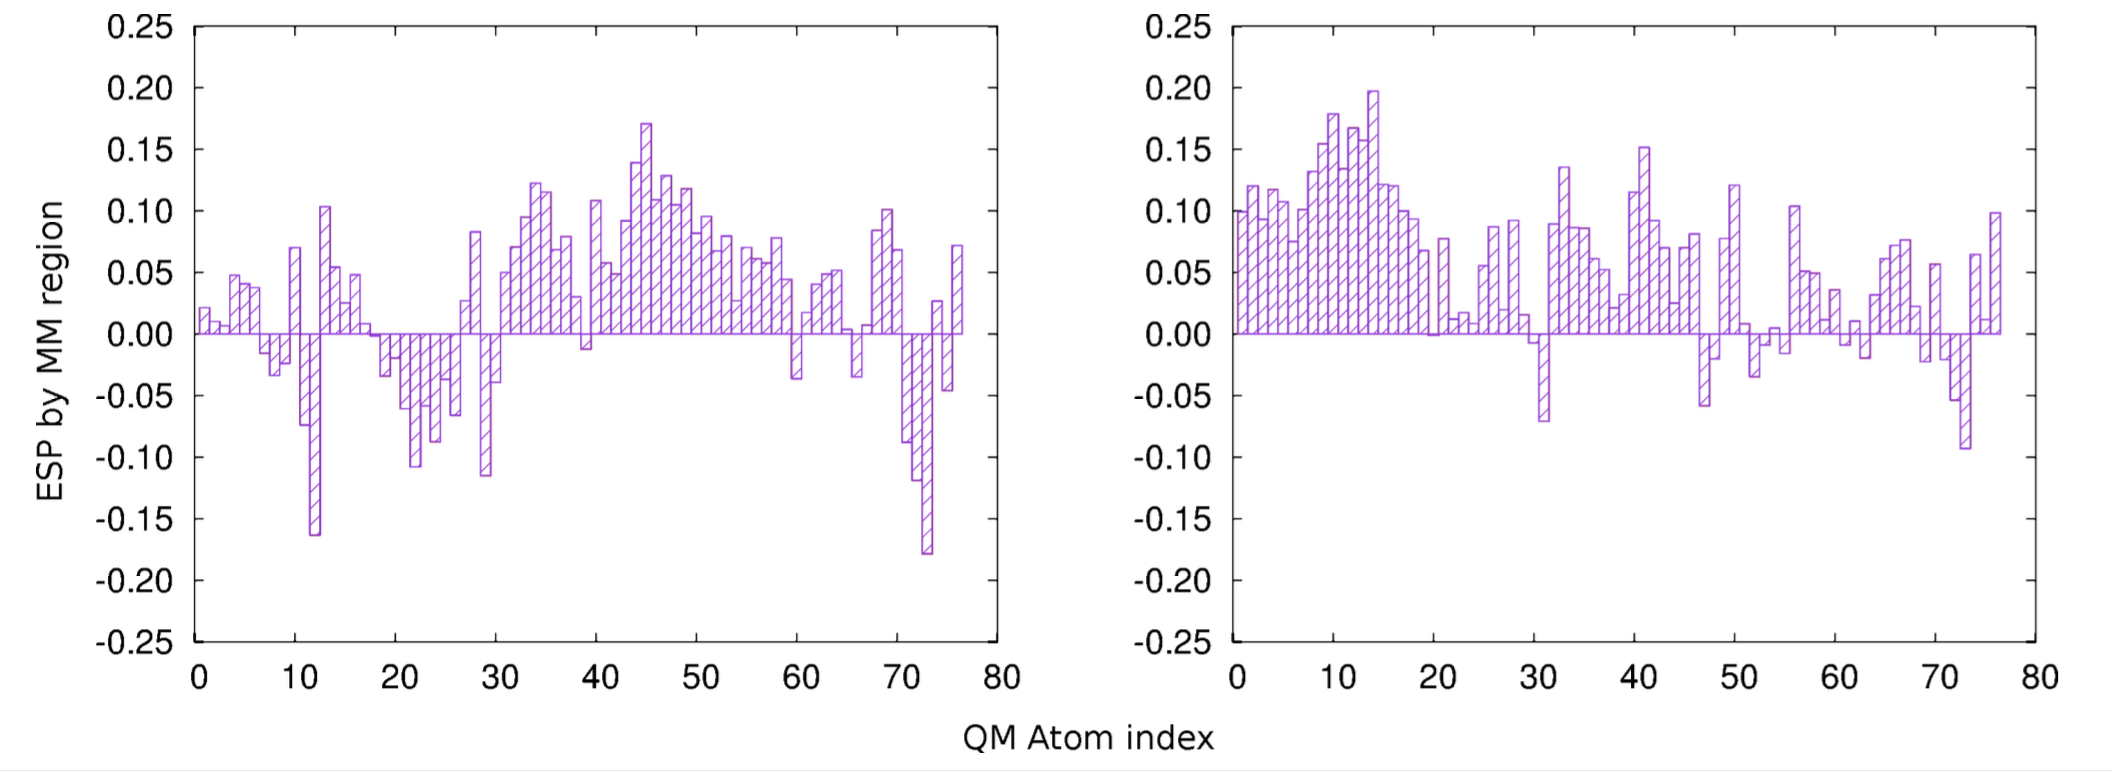
\includegraphics[width=0.8\textwidth,keepaspectratio,natwidth=193,natheight=40]
  {research/sugita/fig03.png}
  \caption{Electrostatic potential on QM atoms of the reactant state in
 the model crowding environment (left) and solution (right). QM atom
 index 43-55 corresponds to triphosphate moiety of GTP.} 
  \locallabel{fig:fig03}
\end{figure}

\section{Schedule and Future Plan}

So far, GENESIS has been optimized mainly on K computer. In this year or
later, we consider other platforms than K, such as intel CPU cluster,
nvidia GPU processor, and post K. Since these CPU (or GPU) architectures
are quite different with each other, a single MD kernel does not work
well for all the different computational platforms. So, GENESIS will
have multiple kernels that are optimized to one of the computational
platforms. The disadvantage of this approach is that we have more effort
on programming, reducing potential bugs for each kernel, and so on. It
should be hard task for our team, but there is no other good ways to
improve the performance of GENESIS in multiple platforms. 

We would like to simulate more and more large biological systems for
investigating slow biological dynamics. For this purpose, we need to
develop multi-scale and multi-resolution programs that are scalable on K
or post-K computers. Currently, GENESIS/SPDYN is useful for all-atom MD
simulations on these supercomputers, but does not show good performance
on CG-modeling and simulations of biological systems due to the small
number of particles and load-balance problems. We need a new program
that is suitable for such CG-modeling and simulations by introducing a
different parallelization scheme. Such new program, which we call CGDYN,
will be developed soon. 

Another important aspect is the introduction of quantum effect to
investigate the chemical reactions in enzymes. Bond-formation or
breaking can not be simulated by using classical force fields, but
should be investigated by using ab initio Quantum theory. Considering
the large system size in biological systems, only possible approach is
to use QM/MM hybrid calculations. We have a basic QM/MM code for
computing potential energies of QM/MM systems and optimizing the systems
based on the hybrid QM/MM potential energy functions. We plan to extend
the calculations for larger periodic boundary systems and to allow the
reaction calculations in proteins. 

%%% DO NOT EDIT BELOW

\section{Publications}

%\printbibliography[keyword=journal, heading=subbibliography, title={Journal Articles}, prefixnumbers={1-}, resetnumbers=true]
%\printbibliography[keyword=proceedings, heading=subbibliography, title={Conference Papers}, prefixnumbers={2-}, resetnumbers=true]
%\printbibliography[keyword=invited, heading=subbibliography, title={Invited Talks}, prefixnumbers={3-}, resetnumbers=true]
%\printbibliography[keyword=poster, heading=subbibliography, title={Posters and Presentations}, prefixnumbers={4-}, resetnumbers=true]
%\printbibliography[keyword=deliverable, heading=subbibliography, title={Patents and Deliverables}, prefixnumbers={5-}, resetnumbers=true]

\printbibliography[keyword=journal, heading=subbibliography, title={Journal Articles}, resetnumbers=true]
\printbibliography[keyword=proceedings, heading=subbibliography, title={Conference Papers}]
\printbibliography[keyword=invited, heading=subbibliography, title={Invited Talks}]
\printbibliography[keyword=poster, heading=subbibliography, title={Posters and Presentations}]
\printbibliography[keyword=deliverable, heading=subbibliography, title={Patents and Deliverables}]

\end{refsection}
